\documentclass{beamer}

\mode<presentation>
{
  \usetheme{Madrid}
  \usecolortheme{beaver}
  \usefonttheme{serif}
  \setbeamertemplate{navigation symbols}{}
  \setbeamertemplate{caption}[numbered]
} 

\usepackage[english]{babel}
\usepackage[utf8x]{inputenc}
\usepackage{bbm}

\usepackage{pgfpages}
\pgfpagesuselayout{resize to}[physical paper width=8in, physical paper height=6in]

\title[An enhanced version of LLOB model]{Market impact with multi-timescale liquidity}
\author{Junliang Zhou, Likun Ouyang}
\institute{Baruch College, Master of Financial Engineering}
\date{\today}

\begin{document}

\begin{frame}
  \titlepage
\end{frame}

\begin{frame}{Outline}
  \tableofcontents
\end{frame}

\section{Introduction to LLOB model}

\begin{frame}{Introduction to LLOB model}
  \tableofcontents[currentsection]
\end{frame}

\begin{frame}{Introduction to LLOB model}

The latent volume densities of limit orders in the order book $\phi_\text{b}(x,t)$ (bid side) and $\phi_\text{a}(x,t)$ (ask side) follows
\begin{equation}\label{llobpde1}
\begin{split}
\partial_t\phi_\text{b} &= D\partial_{xx}\phi_\text{b}-\nu\phi_\text{b}+\lambda\Theta(x_t-x)-R_\text{ab}(x) \\
\partial_t\phi_\text{a} &= D\partial_{xx}\phi_\text{a}-\nu\phi_\text{a}+\lambda\Theta(x-x_t)-R_\text{ab}(x)
\end{split}
\end{equation}

The price $x_t$ is defined as the solution of
\begin{equation}\label{llobpde2}
\begin{split}
&\phi(x_t,t) = \phi_\text{b}(x,t)-\phi_\text{a}(x,t)=0 \\
&\partial_t\phi = D\partial_{xx}\phi-\nu\phi+\lambda\text{sign}(x_t-x)
\end{split}
\end{equation}

\end{frame}

\begin{frame}{Introduction to LLOB model}

The stationary order book is given by 
\begin{equation}
\phi^\text{st}(\xi) = -\frac{\lambda}{\nu}\text{sign}(\xi)\left[1-\exp\left(-\frac{|\xi|}{\xi_c}\right)\right]
\end{equation}

where $\xi_c =\sqrt[]{D\nu^{-1}}$ and $\xi=x-x_t$.

\begin{figure}
\centering
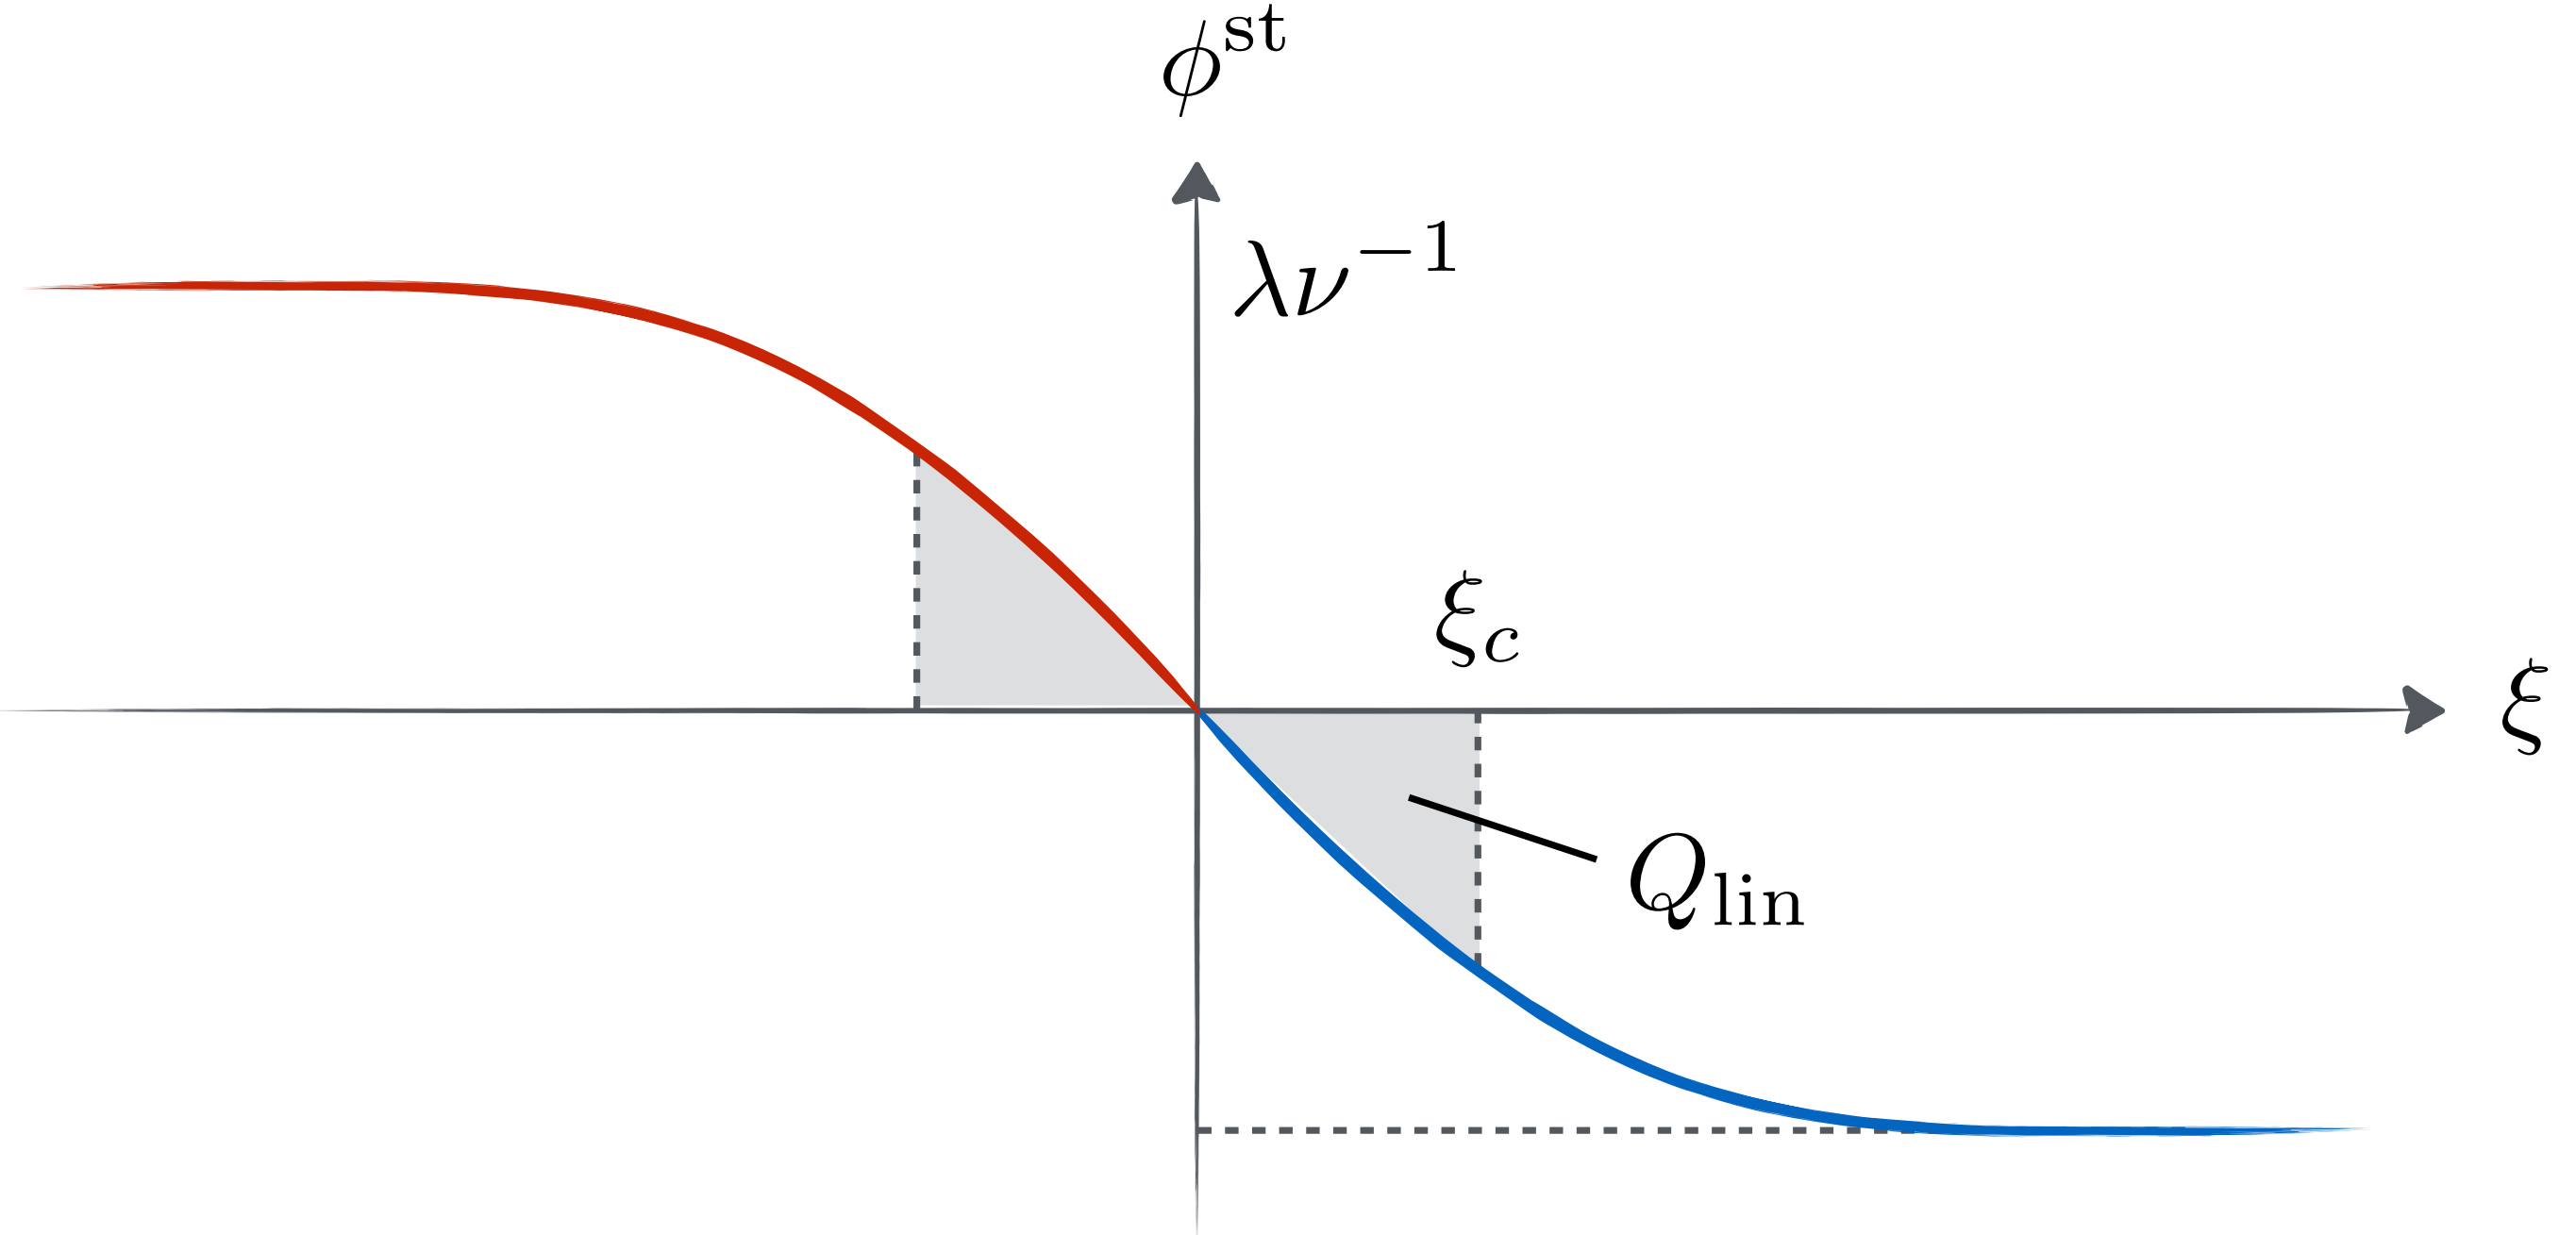
\includegraphics[width=0.6\textwidth]{figure1.PNG}
\caption{\label{fig:f1}Stationary order book under LLOB model.}
\end{figure}

\end{frame}

\subsection{Deficiencies of LLOB model}

\begin{frame}{Deficiencies of LLOB model}

\begin{itemize}
\item The original LLOB model focused on the infinite memory limit, namely $\nu, \lambda \to 0$ while keeping $\mathcal{L} \sim \lambda \nu^{-1/2}$ constant, such that the latent order book becomes exactly linear since in that limit $\xi_c \to \infty$; while in reality we are facing finite memory. \newline
\item A strict square-root law is only recovered in the limit where the execution rate $m_0$ of the meta-order is larger than the normal execution rate $J$ of the market itself; whereas most meta-order impact data is in the opposite limit $m_0 \lesssim 0.1J$. \newline
\item The theoretical inverse square-root impact decay is too fast and leads to significant short time mean-reversion effects, not observed in real prices.
\end{itemize}

\end{frame}

\section{Market impact profile under finite memory}

\begin{frame}{Price and impact profile under finite memory}
  \tableofcontents[currentsection]
\end{frame}

\begin{frame}{Price and impact profile under finite memory}

We introduce a buy meta-order as the source of market impact with intensity rate $m_t$, then equation (\ref{llobpde2}) becomes
\begin{equation}\label{llobpde3}
\partial_t\phi = D\partial_{xx}\phi-\nu\phi+\lambda\text{sign}(x_t-x)+m_t\delta(x-x_t)\mathbbm{1}_{[0,T]}
\end{equation}

Focusing on constant participation rates $m_t=m_0$, we consider

\begin{itemize}
\item Small participation rate $m_0\ll J$ \textit{v.s.} large participation rate $m_0\gg J$.
\item Fast execution $\nu T\ll 1$ \textit{v.s.} slow execution $\nu T\gg 1$.
\item Small meta-order volumes $Q=m_0 T\ll Q_\text{lin}$ \textit{v.s.} large meta-order volumes $Q=m_0 T\gg Q_\text{lin}$.
\end{itemize}

\end{frame}

\subsection{Price trajectories with finite cancel and deposit rates}

\begin{frame}{Price trajectories with finite cancel and deposit rates}

For fast execution and small meta-order volumes, we have the price trajectory as
\begin{equation}
x_t=\alpha\left[z_t^0+\sqrt[]{\nu}z_t^1+\mathcal{O}(\nu)\right]
\end{equation}

While for slow execution and/or large meta-order volumes,
\begin{equation}
x_t=\frac{m_0\nu}{\lambda}t
\end{equation}

\end{frame}

\begin{frame}{Price trajectories with finite cancel and deposit rates}

\begin{figure}
\centering
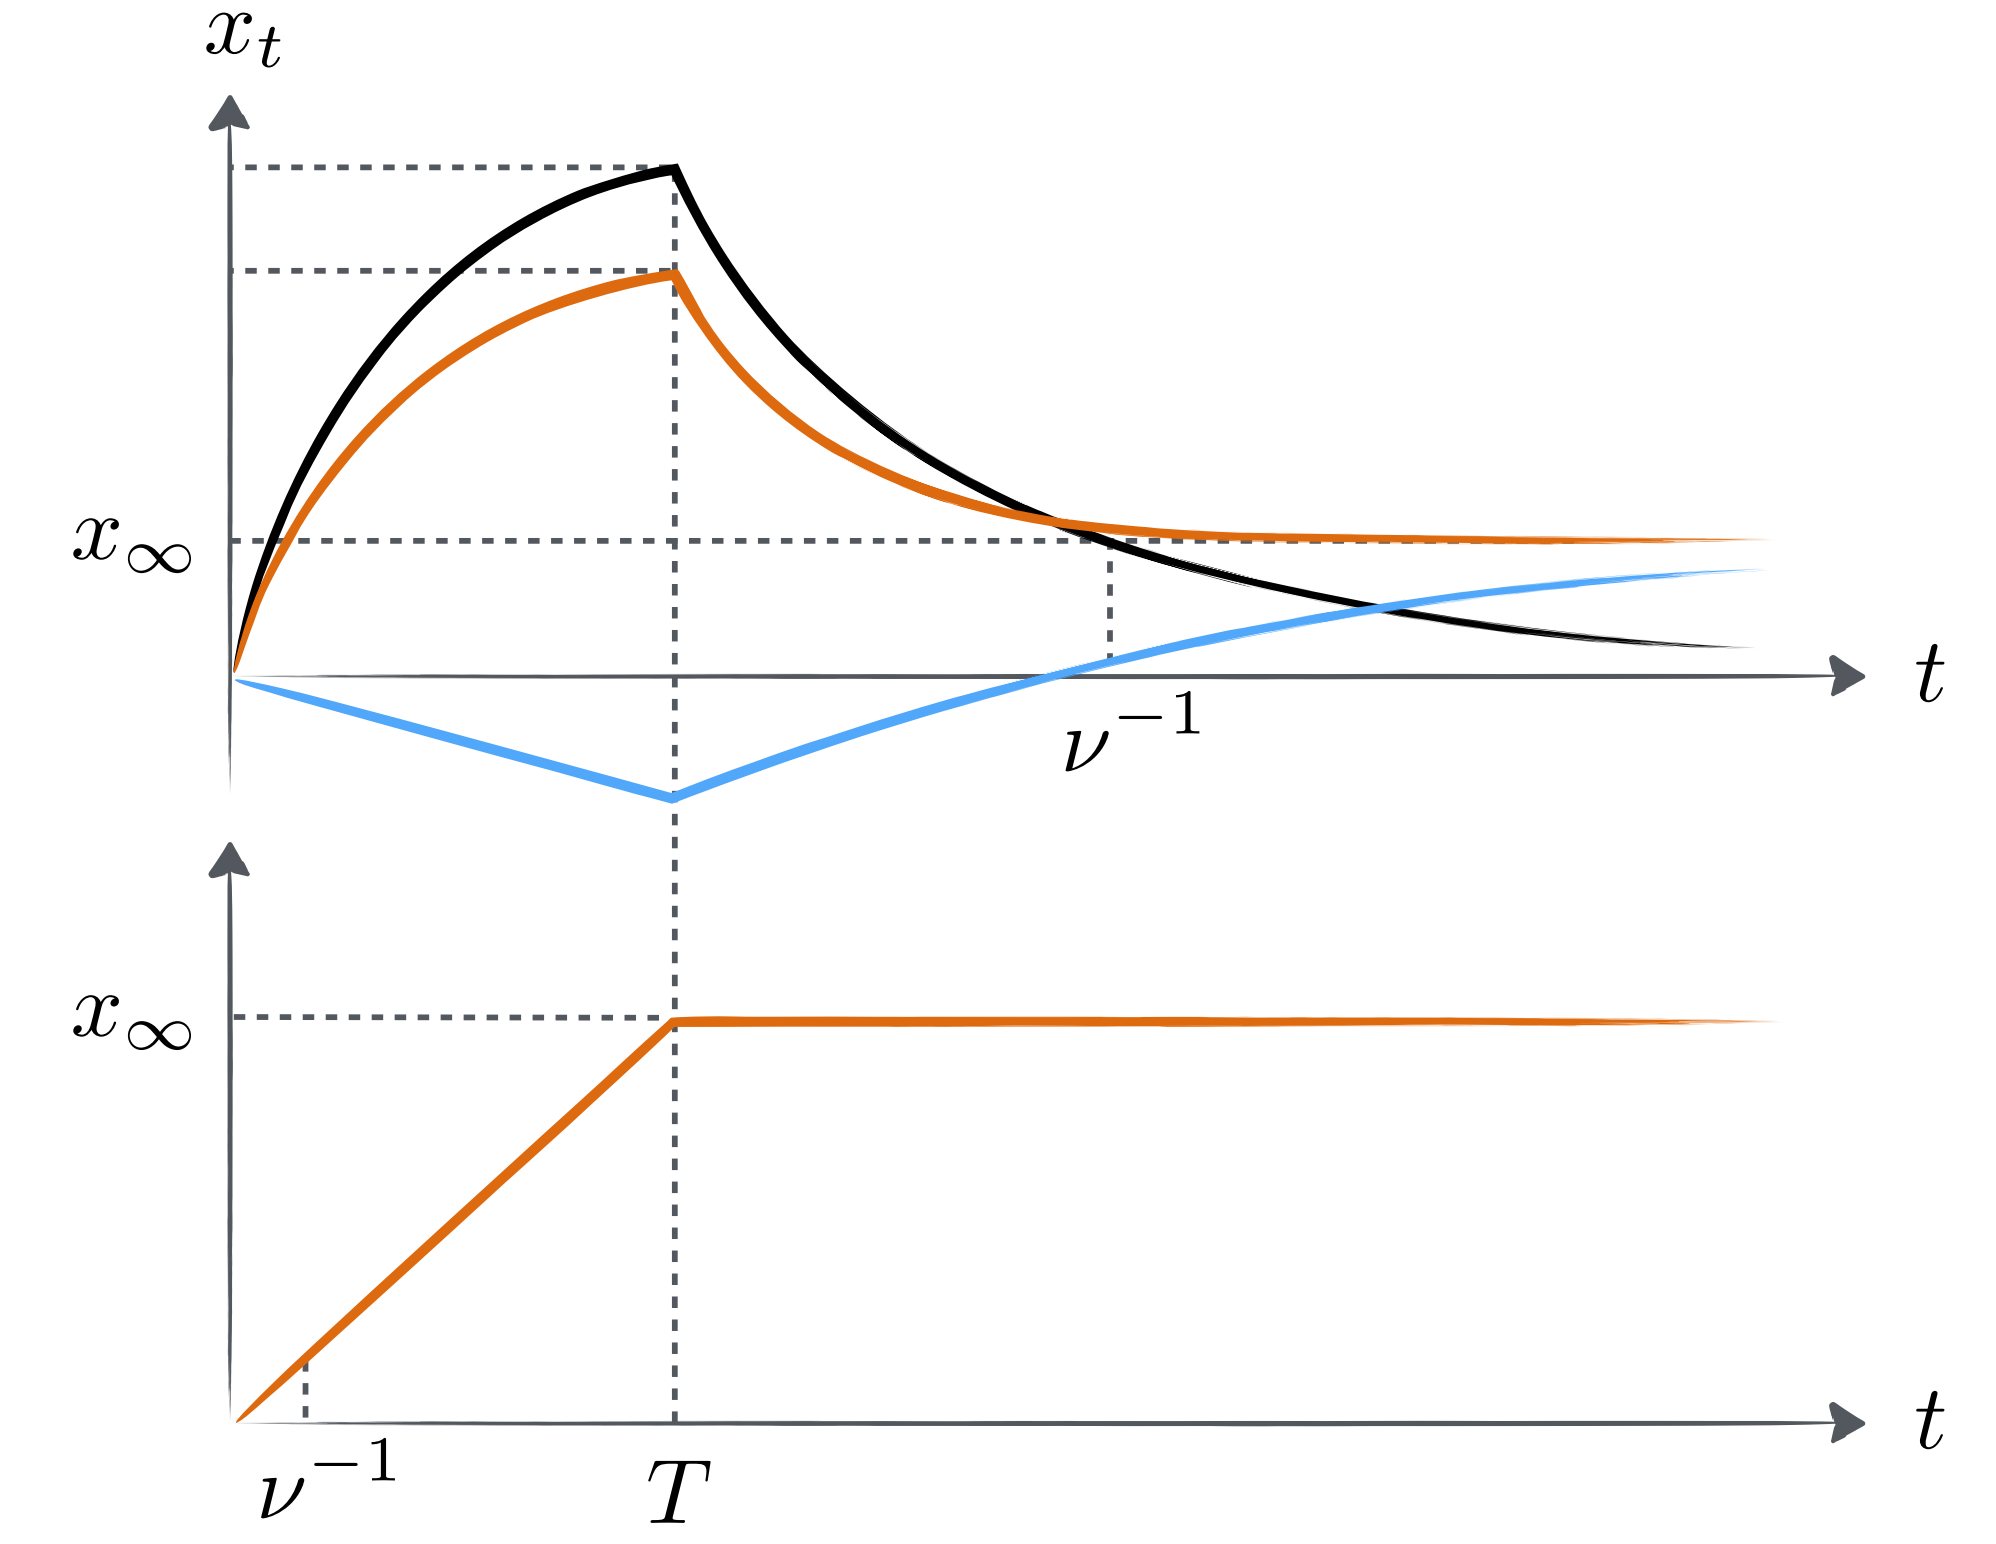
\includegraphics[width=0.6\textwidth]{figure2.PNG}
\caption{\label{fig:f2}Top graph: Price trajectory during and after a buy meta-order execution for $\nu T \ll 1$. Bottom graph: Price trajectory for $\nu T \gg 1$.}
\end{figure}

\end{frame}

\subsection{Linear permanent impact with finite memory}

\begin{frame}{Linear permanent impact with finite memory}

We find that the permanent impact $I_\infty$ follows
\begin{equation}
I_\infty=\frac12\xi_c\frac{Q}{Q_\text{lin}}
\end{equation}

which is linear in execution volume $Q$ in both small and large participation regime. (see to $x_\infty$ in Figure \ref{fig:f2}) \newline

The result is dictated by non-arbitrage arguments and compatible with the classical Kyle model.

\end{frame}

\section{The double-frequency framework}

\begin{frame}{The double-frequency framework}
  \tableofcontents[currentsection]
\end{frame}

\begin{frame}{The double-frequency framework}
Consider there are two sorts of agents co-exists in the market:

\begin{itemize}
\item Slow agents with vanishing cancellation and deposition rates: $\nu_\text{s} T \to 0$, while keeping the corresponding liquidity $\mathcal{L}_\text{s} := \lambda_\text{s}/\sqrt[]{\nu_\text{s} D}$ finite.
\item Fast agents with large cancellation and deposition rates: $\nu_\text{f} T \gg 1$, such that $\mathcal{L}_\text{f} := \lambda_\text{f} / \sqrt[]{\nu_\text{f} D} \gg \mathcal{L}_\text{s}$.
\end{itemize}

\end{frame}

\subsection{LLOB model with fast and slow agents}

\begin{frame}{LLOB model with fast and slow agents}

$\phi_\text{s}$ and $\phi_\text{f}$ follows equation (\ref{llobpde3}) with their own coefficients $\nu,\lambda,m_t$ respectively. With the conditions below,
\begin{equation}\label{doublecondition}
\begin{split}
m_{\text{s}t}&+m_{\text{f}t}=m_0 \\
x_{\text{s}t}&=x_{\text{f}t}=x_t
\end{split}
\end{equation}

Then the total order book volume is given by
\begin{equation}
\phi^\text{st}(x) = \phi_\text{s}^\text{st}(x)+\phi_\text{f}^\text{st}(x)
\end{equation}

where
\begin{equation}
\begin{split}
\phi_\text{s}^\text{st} &\approx -\mathcal{L}_\text{s}x \\
\phi_\text{f}^\text{st} &\approx -\frac{\lambda_\text{f}}{\nu_\text{f}}\text{sign}(x)
\end{split}
\end{equation}

\end{frame}

\begin{frame}{LLOB model with fast and slow agents}

\begin{figure}
\centering
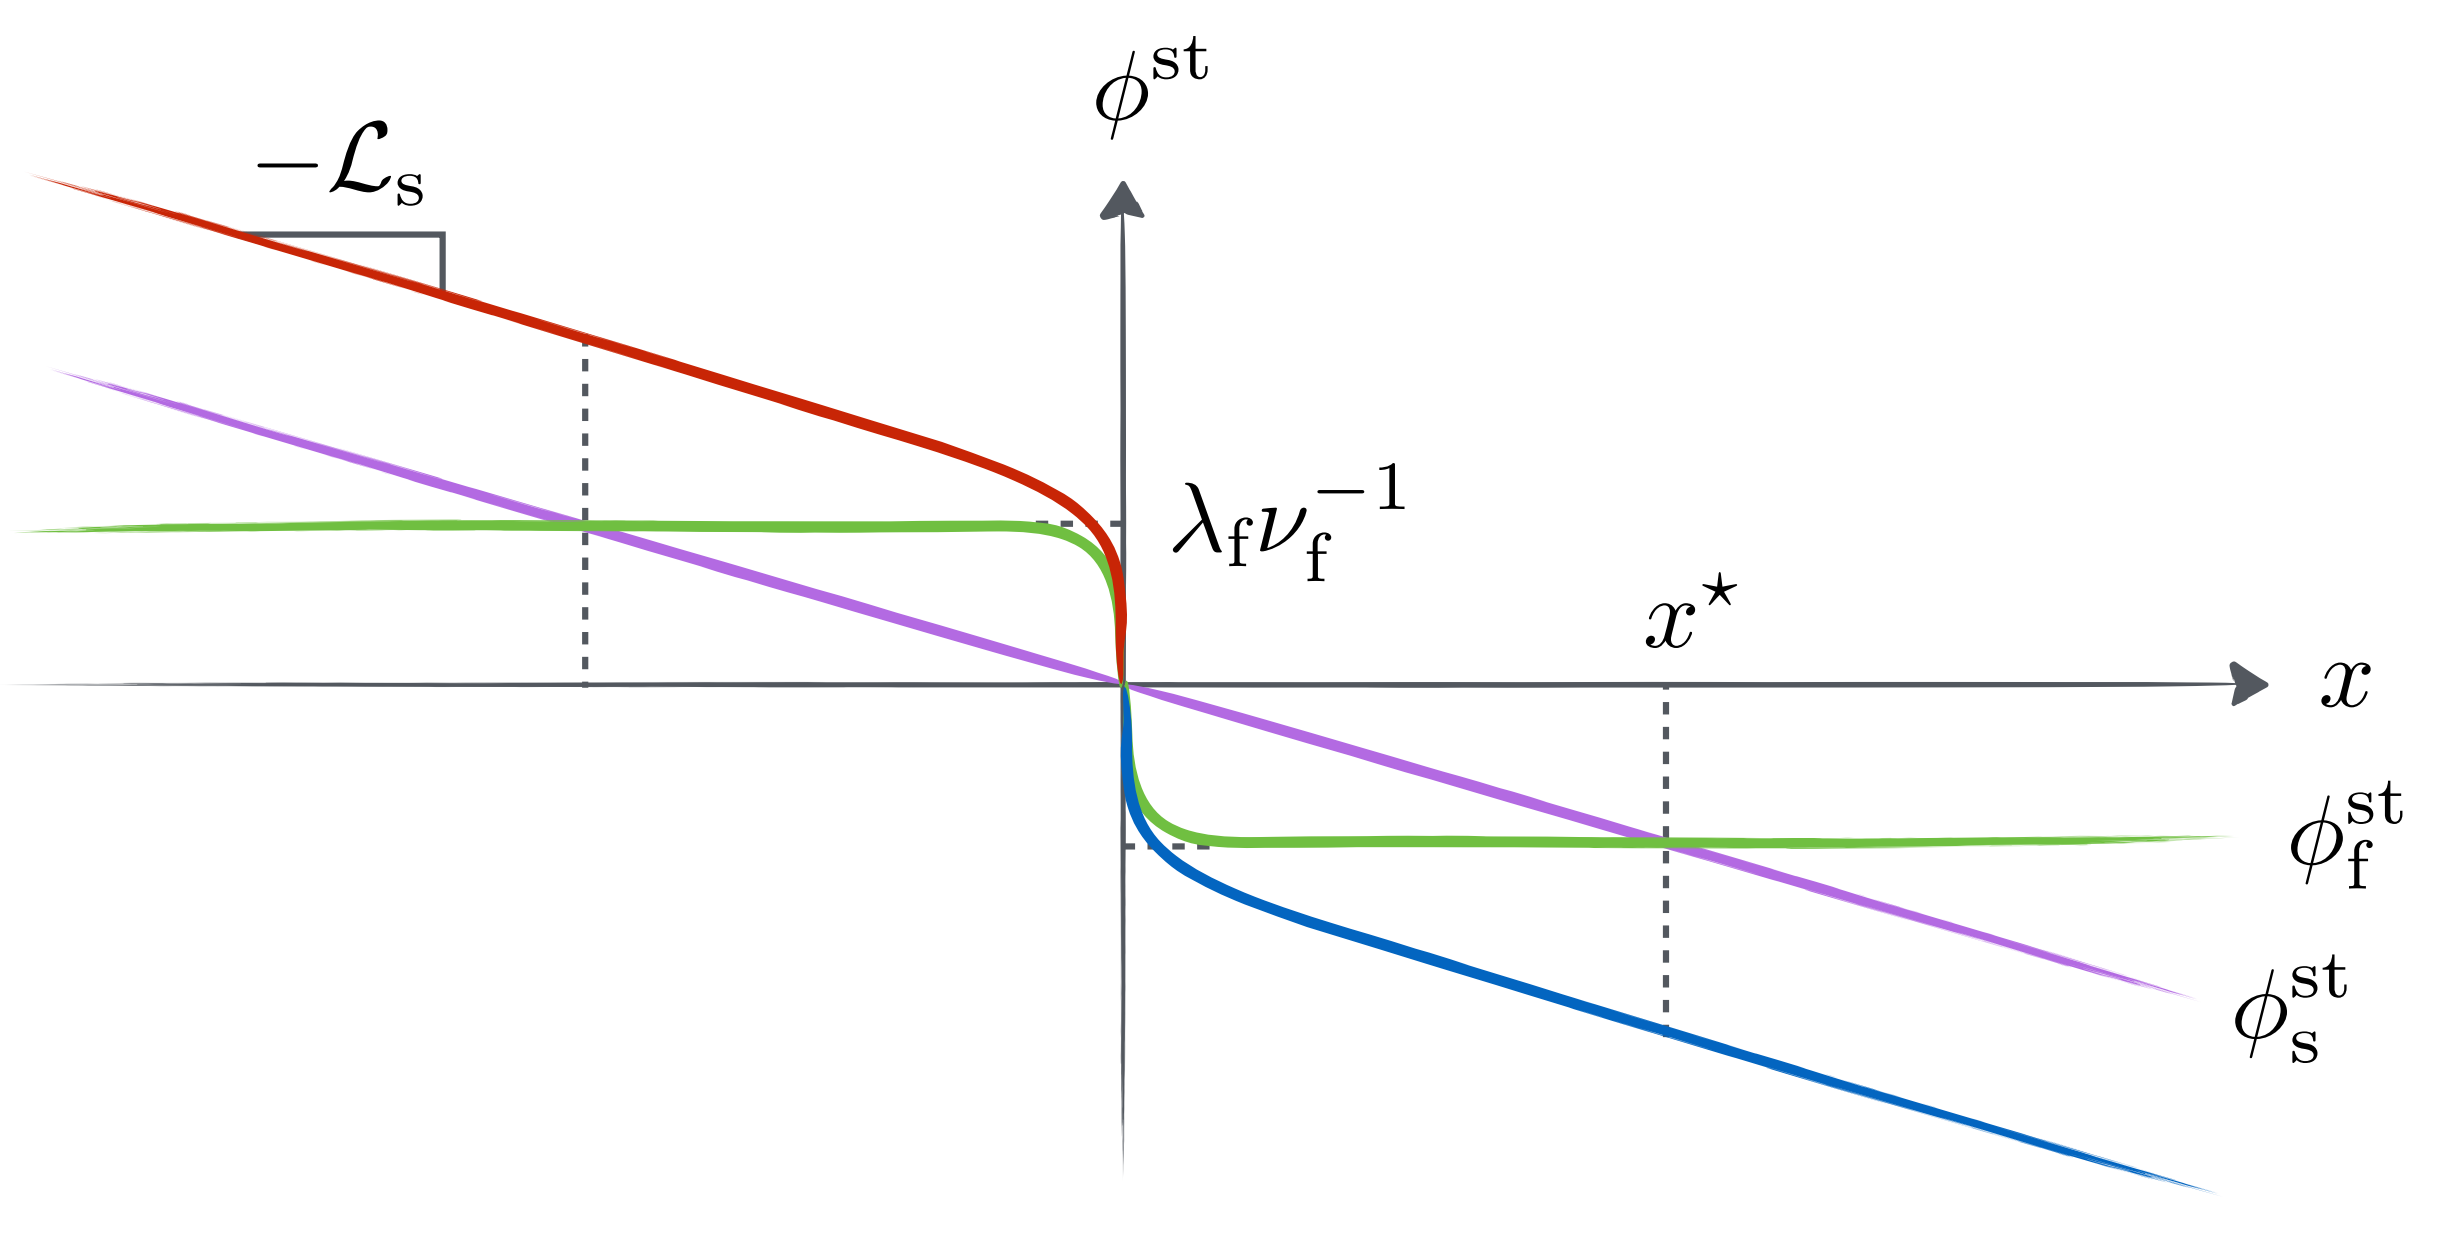
\includegraphics[width=0.6\textwidth]{figure3.PNG}
\caption{\label{fig:f3}Stationary double-frequency order book.}
\end{figure}

\end{frame}

\subsection{From linear to square-root impact}

\begin{frame}{From linear to square-root impact}

Consider the meta-order intensity is large compared to the the average transaction rate of slow traders while small compared to the total transaction rate of the market. That is $J_\text{s}\ll m_0\ll J_\text{f}$. \newline

Equation (\ref{llobpde3}) and equation (\ref{doublecondition}) yield that
\begin{equation}
\begin{split}
m_{\text{f}t} &= \frac{m_0}{\sqrt[]{1+\frac{t}{t^\star}}},\quad t^\star:=\frac{1}{2\nu_\text{f}}\frac{J_\text{f}^2}{J_\text{s}m_0} \\
m_{\text{s}t} &= m_0-m_{\text{f}t}
\end{split}
\end{equation}

\end{frame}

\begin{frame}{From linear to square-root impact}

The resulting price trajectory reads
\begin{equation}
x_t=\frac{\lambda_\text{f}}{\mathcal{L}_\text{s}\nu_\text{f}}\left(\sqrt[]{1+\frac{t}{t^\star}}-1\right)
\end{equation}

The most of the incoming meta-order is executed against the rapid agents for $t<t^\star$ but the slow agents then take over for $t>t^\star$. \newline

The result leads to a market impart that crosses over from a linear regime when $t\ll t^\star$ to a square root regime for $t\gg t^\star$. \newline

The impact decay behaves asymptotically ($t\gg T$) to zero as $x_t\sim t^{-1/2}$.

\end{frame}

\begin{frame}{From linear to square-root impact}

\begin{figure}
\centering
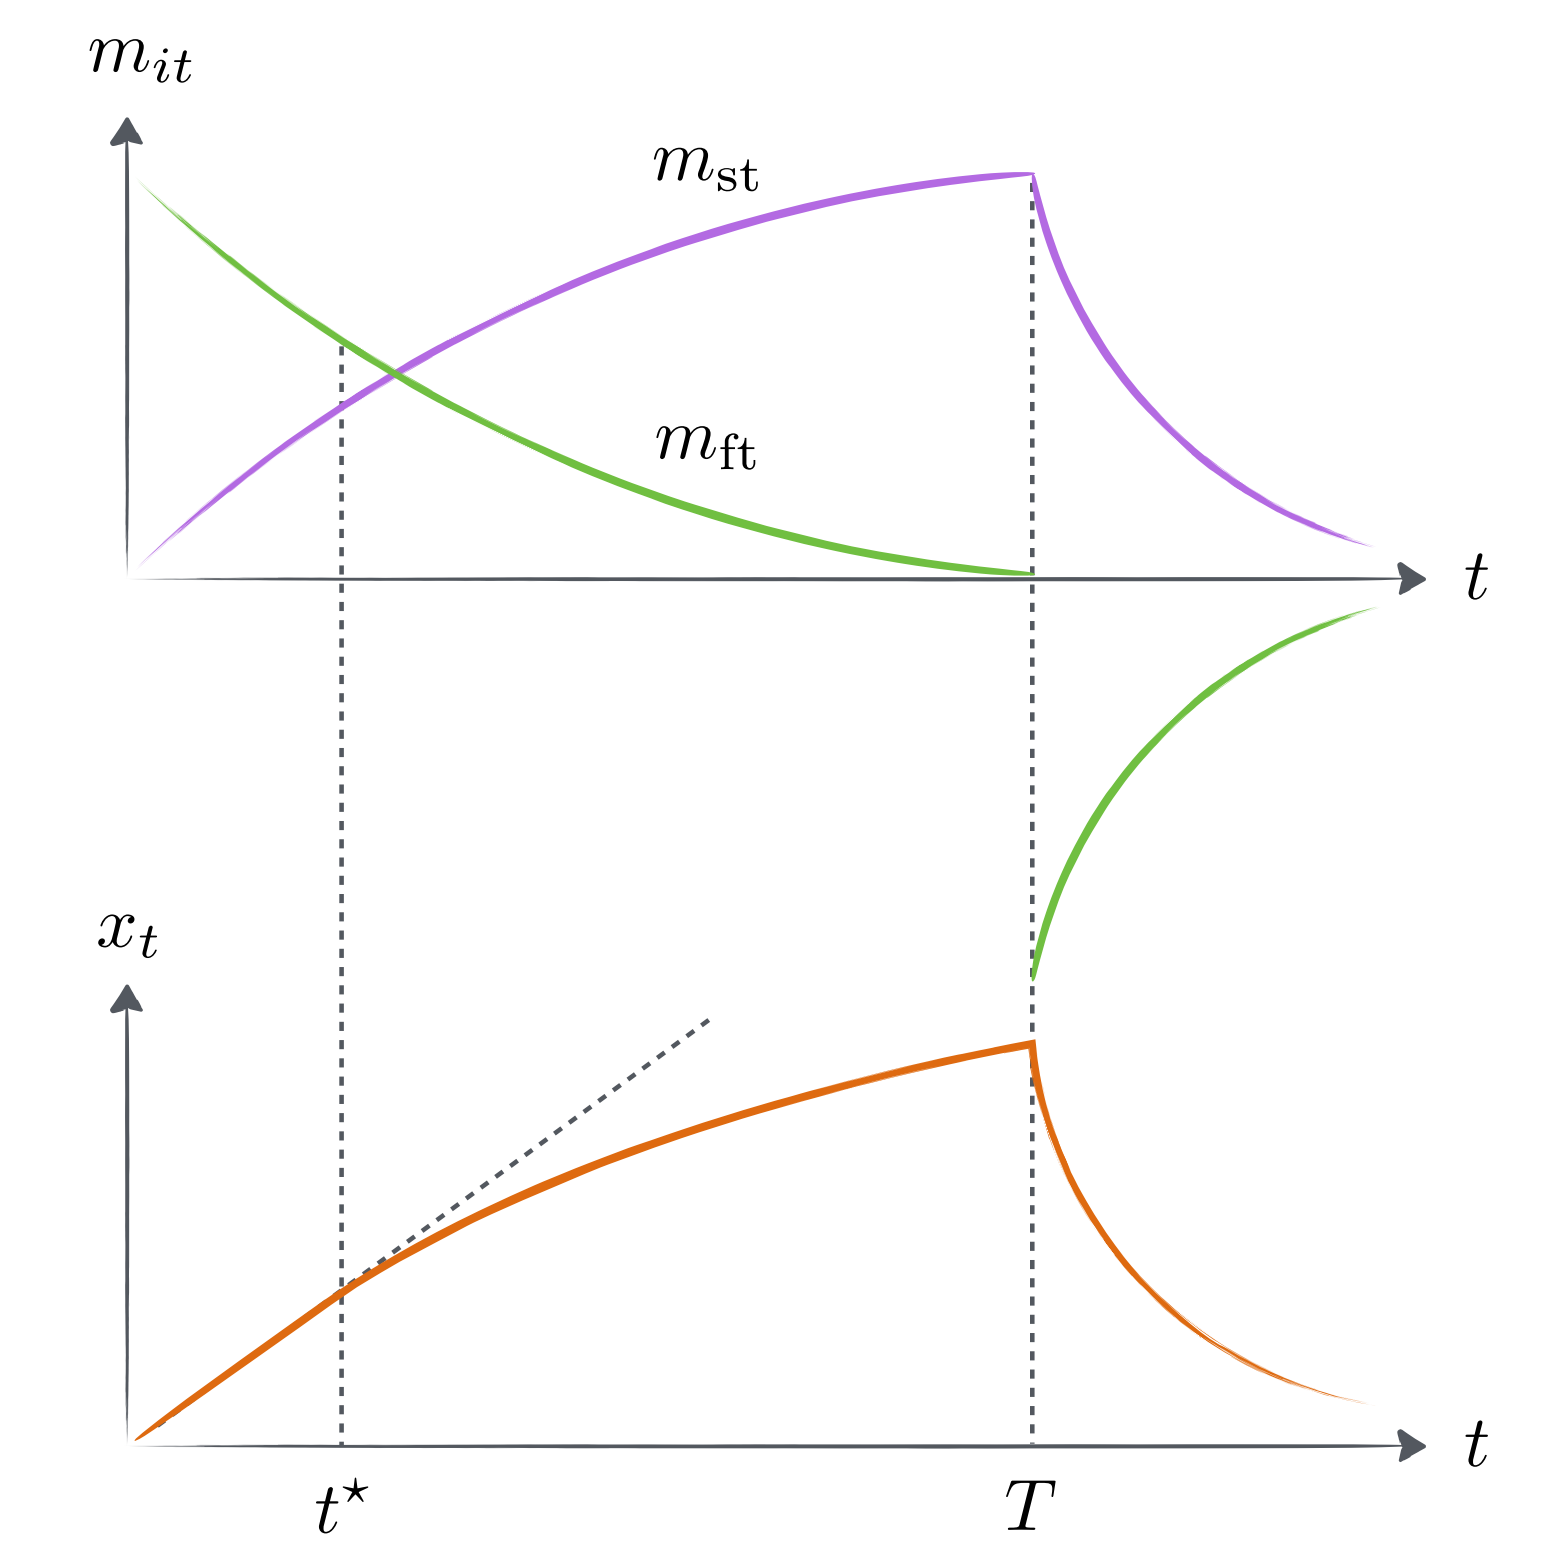
\includegraphics[width=0.5\textwidth]{figure4.PNG}
\caption{\label{fig:f4}Execution rates $m_{it}$ (top) and price trajectory (bottom) within the double-frequency order book model.}
\end{figure}

\end{frame}

\section{The multi-frequency framework}

\begin{frame}{The multi-frequency framework}
  \tableofcontents[currentsection]
\end{frame}

\begin{frame}{The multi-frequency framework}

The double-frequency framework can be extended to the more realistic case of a continuous range of cancellation and deposition rates. 
\begin{equation}\label{multifrequency}
\partial_t{\phi_{\nu}} = D\partial_{xx}{\phi_{\nu}} - \nu \phi_{\nu} + \lambda_{\nu} \text{sign}(x_{\nu t}-x) + m_{\nu t}\delta(x - x_{\nu t})
\end{equation}

where $\phi_{\nu}(x,t)$ denotes the contribution of agents with typical frequency $\nu$ to the latent order book and $\lambda_{\nu} = \mathcal{L}_{\nu}\,\sqrt[]{\nu D}$. \newline 
 
Equation (\ref{multifrequency}) must then be completed with:
\begin{equation}
\begin{split}
&\int_0^{\infty}{\rho(\nu) m_{\nu t} \text{d}\nu} = m_t \\
&x_{\nu t} = x_t, \quad \forall \nu
\end{split}
\end{equation}

where $\rho(\nu)$ denotes the distribution of cancellation rates $\nu$, and where we have allowed for an arbitrary order flow $m_t$.

\end{frame}

\subsection{Resolution of the "diffusivity puzzle"}

\begin{frame}{Resolution of the "diffusivity puzzle"}

With $\langle x^2_t \rangle \propto t^{1-\gamma}$, the latent liquidity in the LLOB case is too persistent and prevents the price from diffusing. \newline

With the power-law distribution $\rho(\nu)$ as
\begin{equation}
\rho(\nu)=Z\nu^{\alpha-1}e^{-\nu t_c}
\end{equation}

The price diffusion under multi-frequency framework is given by
\begin{equation}
\langle x_t^2 \rangle \propto t^{1+2\alpha-\gamma}
\end{equation}

When the liquidity memory times are themselves fat-tailed, mean-reversion effects induced by a persistent order book can exactly offset trending effects induced by a persistent order flow.

\end{frame}

\subsection{Meta-order impact}

\begin{frame}{Meta-order impact}

\begin{figure}
\centering
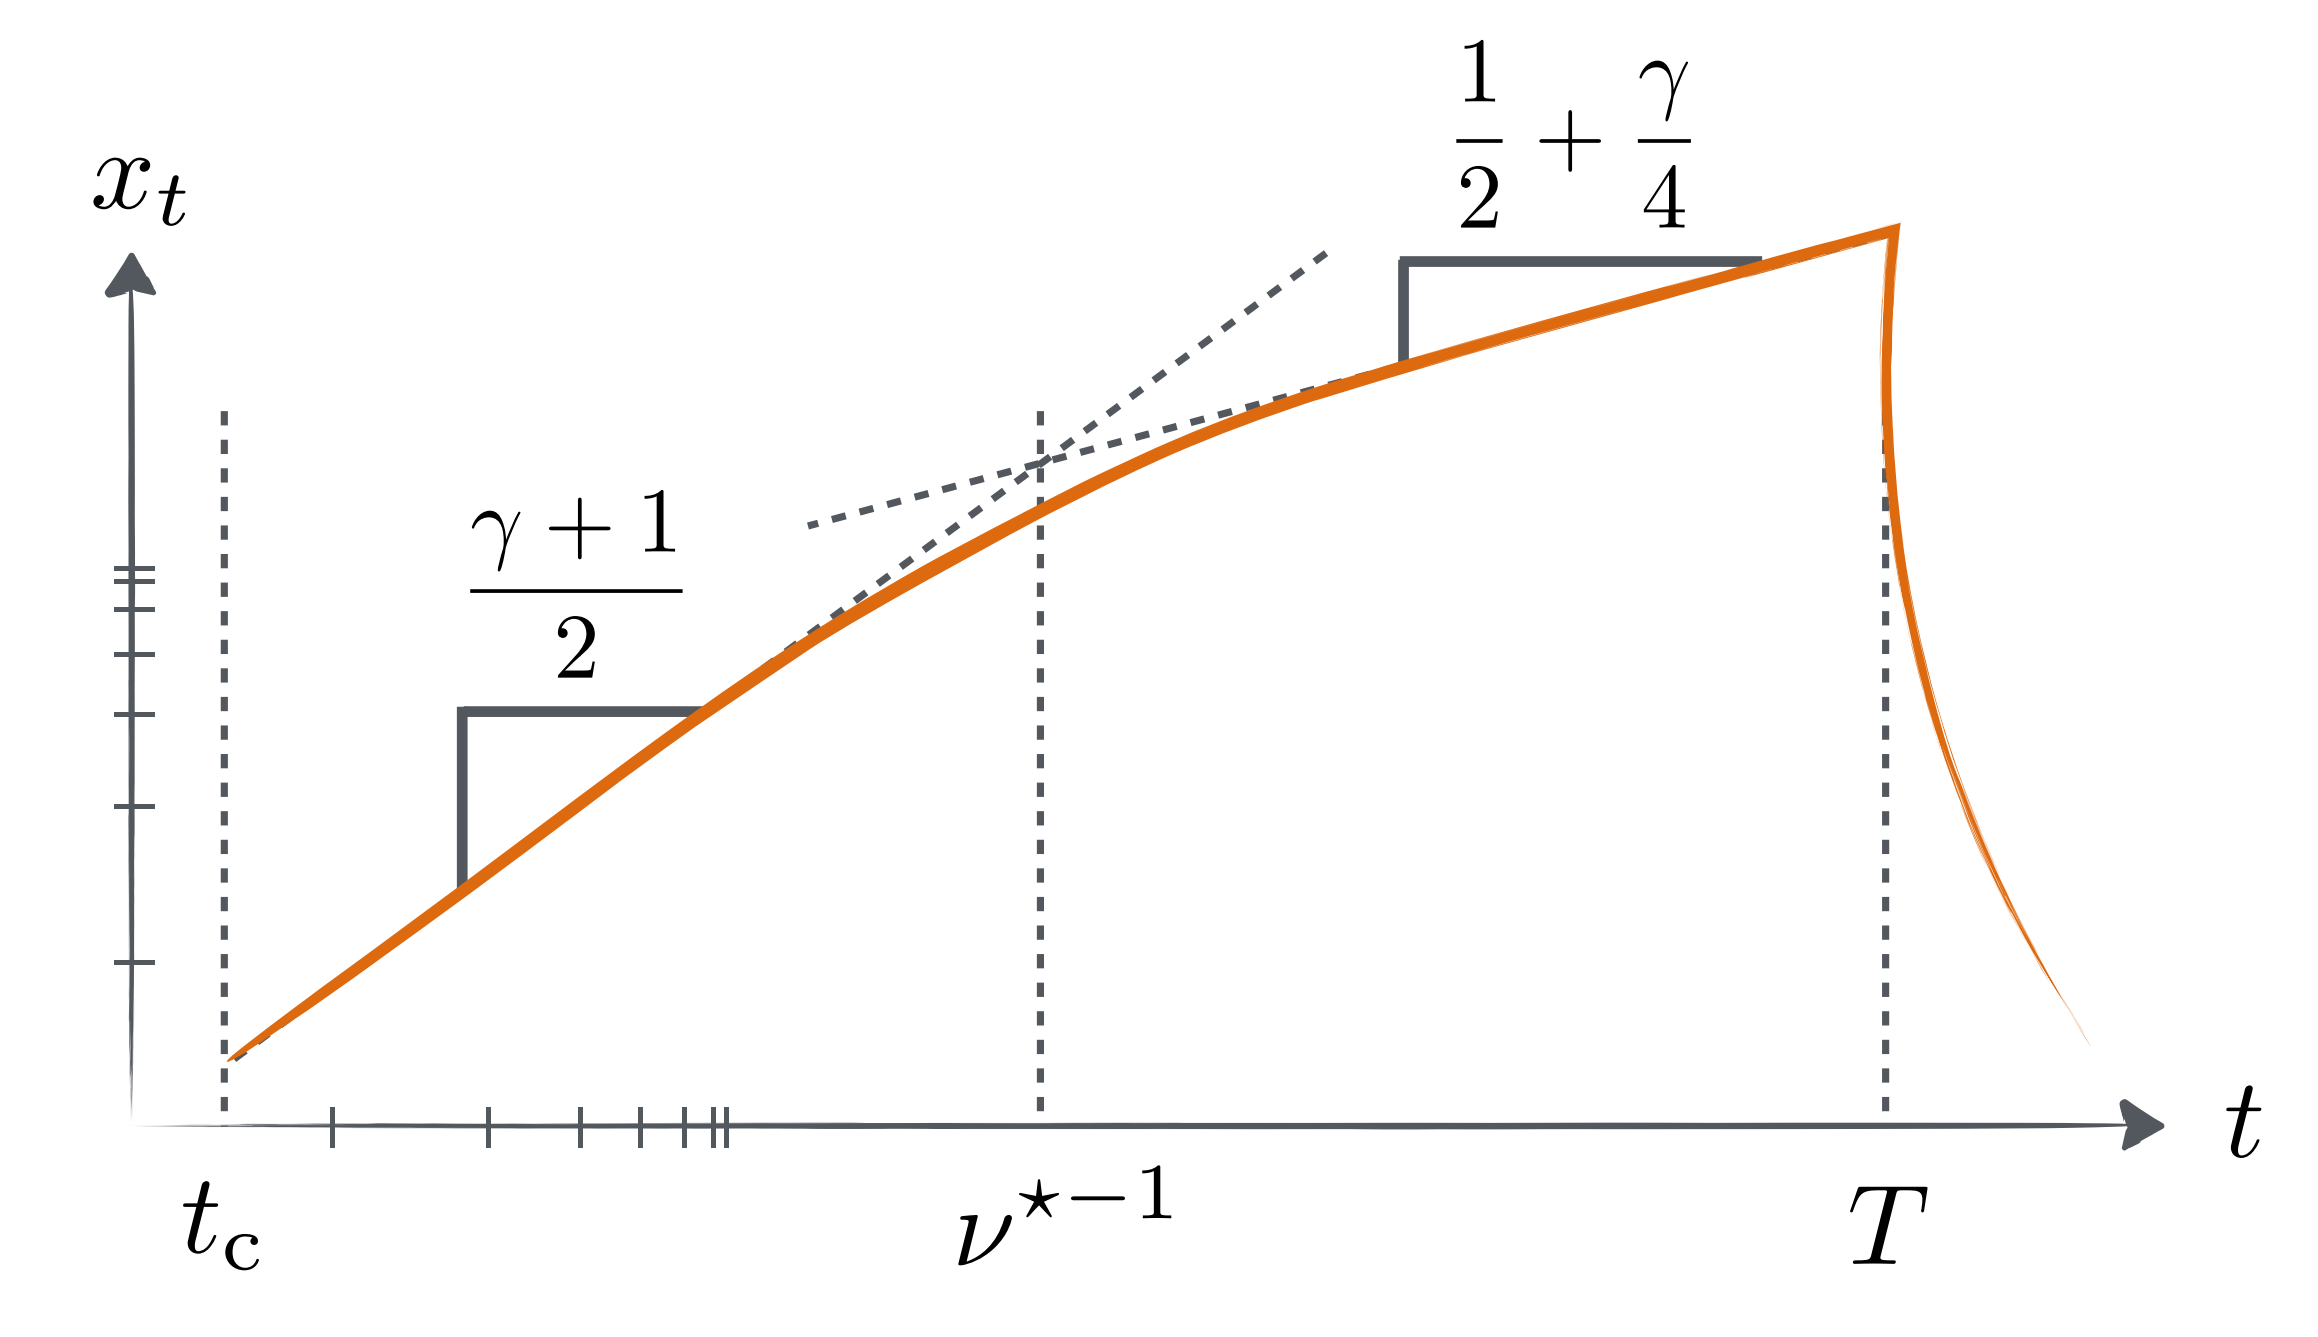
\includegraphics[width=0.6\textwidth]{figure6.PNG}
\caption{\label{fig:f6}  Price trajectory during a constant rate meta-order execution within the multi-frequency order book model. For $\gamma = 1/2$, the impact crosses over from a $t^{3/4}$ to a $t^{5/8}$ regime.}
\end{figure}

\end{frame}

\begin{frame}

\frametitle{References}
\footnotesize{
\begin{thebibliography}{99} 
\bibitem[BOUCHAUD, 2017]{p1} M. Benzaquen and J.P. Bouchaud (2017)
\newblock Market impact with multi-timescale liquidity
\end{thebibliography}

\begin{thebibliography}{99} 
\bibitem[BOUCHAUD, 2015]{p2} J. Donier, J. Bonart, I. Mastromatteo, and J.P. Bouchaud (2015)
\newblock A fully consistent, minimal model for non-linear market impact
\end{thebibliography}
}

\end{frame}

\end{document}